\vspace{-.15in}\section{Research Plan and Methodology}
\label{sec:plan}\vspace{-.075in}

% \xxx strengthens the reliability of datacenter 
% computing with a holistic methodology.
This section first proposes the three objectives in this proposal.
% The first two objectives include preliminary results. 

\vspace{-.15in}\subsection{Objective 1: 
preventing big-data leakage with Precise 
IFT}\label{sec:obj1}\vspace{-.075in}

This section presents \paxos performance problem (\S\ref{sec:ift-problem}) 
and \kakute (\S\ref{sec:kakute}).

\vspace{-.15in}
\subsubsection{Problem: existing IFT systems are slow and incomplete for 
big-data} 
\label{sec:ift-problem}\vspace{-.075in}

No IFT system exists for big-data, and
we attribute it to two major challenges.
% performance is slow, reduce two ..by...
First, existing IFT systems incur high performance overhead, especially for 
data-intensive computations. We ran a recent IFT system
Phosphor~\cite{oo14:phosphor} in Spark with a WordCount algorithm on a dataset 
that is merely 200MB, and
observed 128X longer computation time compared with the native Spark execution 
(\chref{sec:bigdata}). The second challenge is on the architecture of 
DISC frameworks.
DISC frameworks usually contain shuffle procedures which redistribute
data across hosts (DISC frameworks' worker nodes).
However, most existing IFT systems ignore dataflows across hosts.
For the few~\cite{cloudfence:raid13} who support cross-host dataflows,
transferring all tags in shuffles consumes excessive network
bandwidth. Therefore, efficient cross-host tag propagation
is crucial but missing in DISC.

\vspace{-.15in}\subsubsection{\kakute: a fast, precise IFT system for big-data} 
\label{sec:kakute}\vspace{-.075in}

\begin{figure}[h]
    \centering
    \begin{minipage}{.48\textwidth}    
        \vspace{-.15in}
        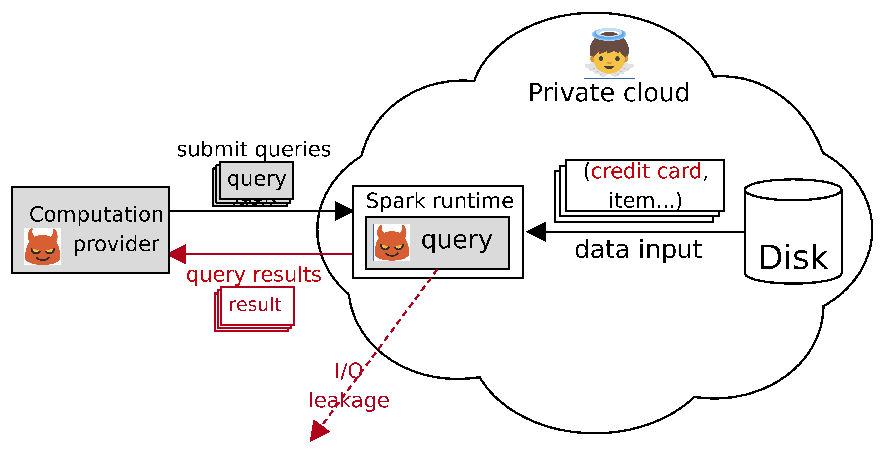
\includegraphics[width=0.31\textheight]{figures/threat_private.ps}
        \vspace{-.3in}         
        \caption{Threat model).}
        \label{fig:falcon-arch}
    \end{minipage}
    \centering
    \begin{minipage}{0.48\textwidth}
        \vspace{-.17in}
        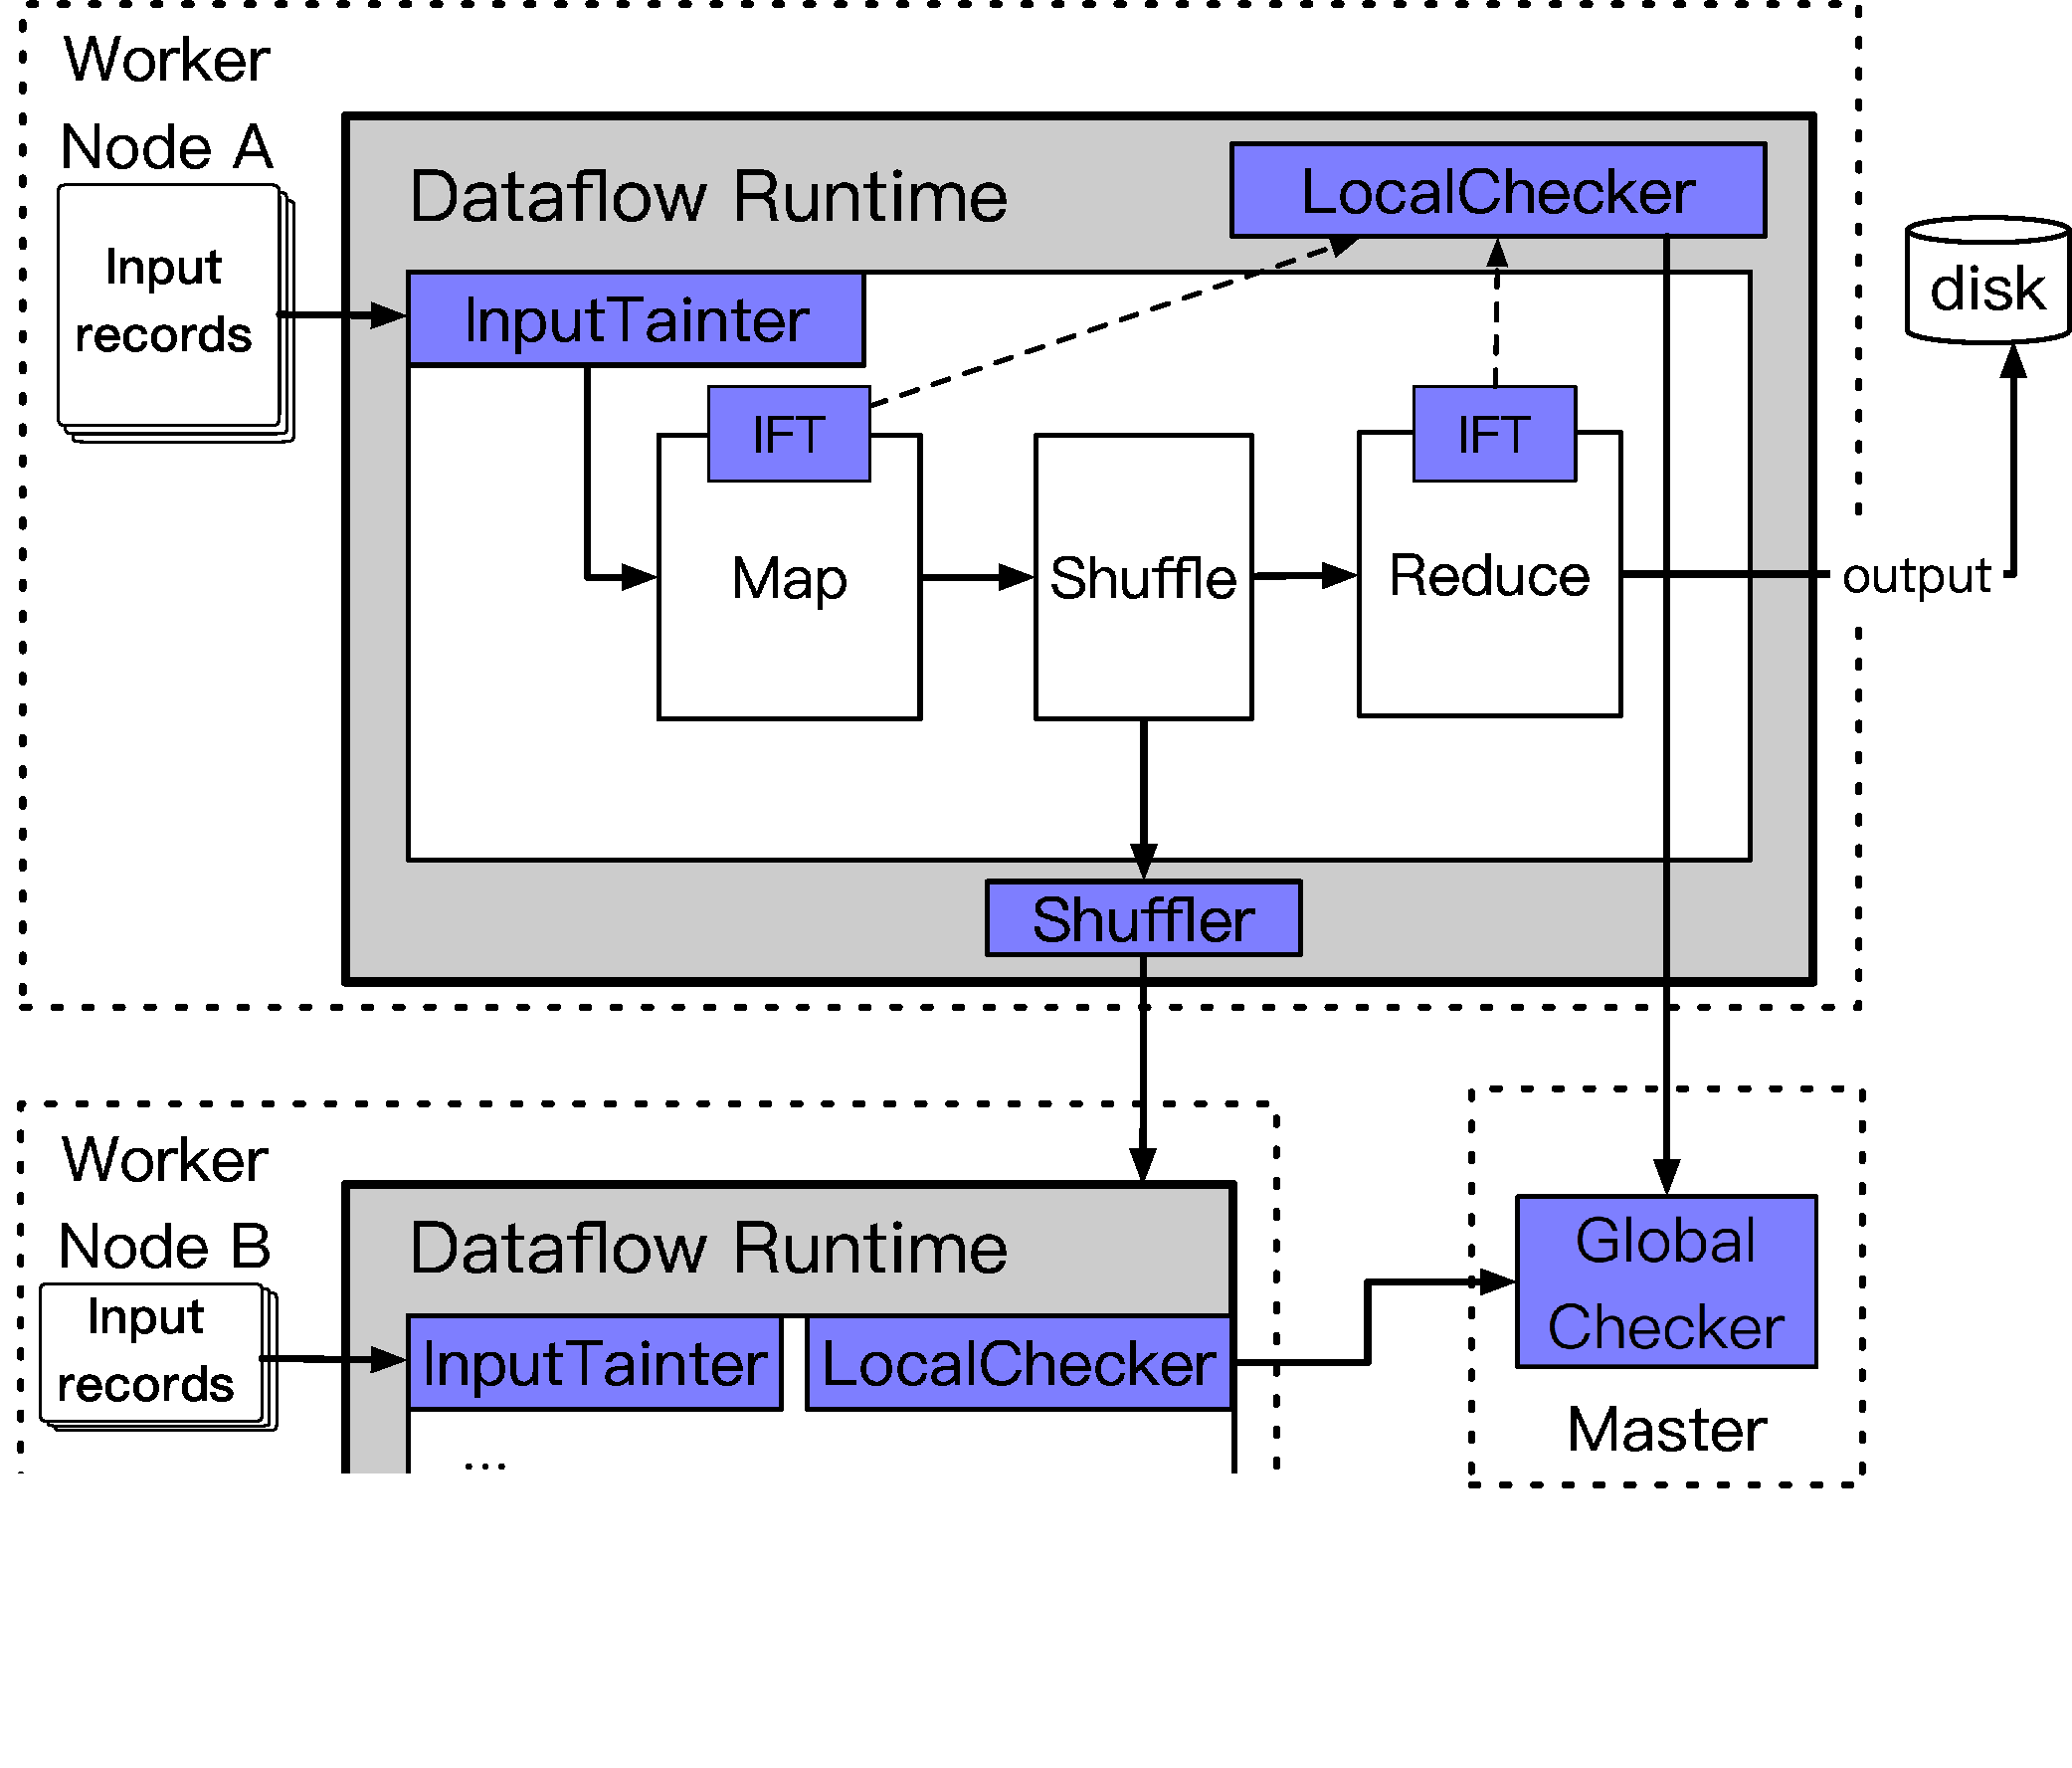
\includegraphics[width=0.34\textheight]{figures/kakute_arch.ps}
        \vspace{-.32in}
        \caption{\kakute architecture.}
        \label{fig:falcon-protocol}
    \end{minipage}
\end{figure}

This paper presents \kakute\footnote{Kakute is a precise, multi-purpose weapon 
used by
Ninja.}, the first precise and fine-grained information flow
analysis system in DISC frameworks.
Our key insight to address the IFT efficiency challenge is that multiple fields 
of a record
often have the same tags.
Leveraging this insight, we present two new techniques, \lazyp and \tagcache.
\lazyp avoids unnecessary tag combinations by only keeping the \textit{lineage 
of tags} in
the same UDF, while \tagcache reduces memory usage by sharing
tags among multiple fields in each record.
To tackle the architecture challenge,
\kakute completely captures dataflows in shuffles, and it efficiently
reduces the amount of transferred IFT tags using \tagcache.

We will implement \kakute in Spark.
We leverage Phosphor~\cite{oo14:phosphor}, an efficient IFT system working
in the Java byte-code level.
\kakute instruments computations of a Spark worker process
to capture dataflow inside user-defined-functions (UDFs).
Dataflow information
is kept in a worker process and \kakute propagates it to other processes while 
shuffling.
Therefore, IFT is completely captured across hosts and processes.
In this paper, DISC frameworks and \kakute are trusted; UDFs are untrusted and 
they
may be malicious or buggy.
\kakute provides different granularities of tracking with two types of tags: 
\func{Integer}
and \func{Object} tags. \func{Integer} provides 32 distinct tags,
which is suitable for detecting information
leakage and performance bugs. \func{Object}
provides an
arbitrary number of tags, which is suitable for
data provenance and programming debugging.
\kakute provides a unified API to tackle diverse problems. Based on this 
unified API, we implemented 4 built-in checkers for \appsn
security and reliability problems: sensitive information leakage, data 
provenance, programming and performance bugs.

\begin{wrapfigure}{r}{7cm}
  \vspace{-.1in}
  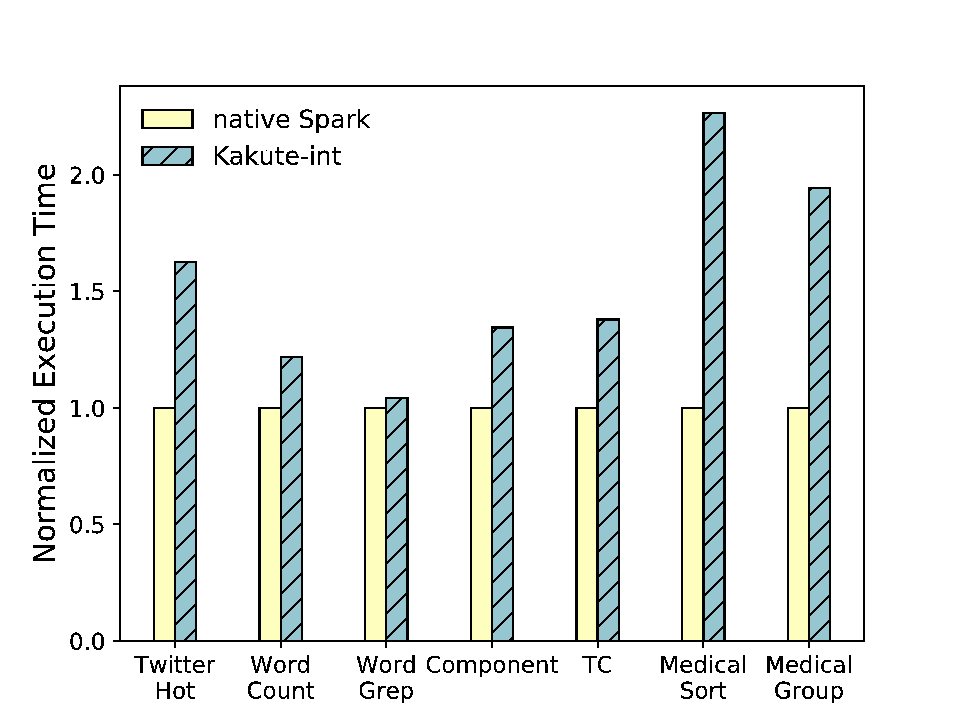
\includegraphics[width=7cm]{figures/time_overhead.ps}\\
  \vspace{-.3in}
  \caption{\kakute execution time normalized to Spark executions.}
  \label{fig:scalability}
\end{wrapfigure}

\para{Preliminary results.} We evaluated \kakute on \appeval diverse 
algorithms, including three text processing
algorithms WordCount~\cite{spark:example}, WordGrep~\cite{newt:socc13} and 
TwitterHot~\cite{spark:example}, two graph algorithms 
TentativeClosure~\cite{spark:example}
and ConnectComponent~\cite{spark:example}, and two medical analysis programs 
MedicalSort~\cite{pigmix} and MedicalGroup~\cite{pigmix}.
These algorithms cover
all big-data algorithms evaluated in two related 
papers~\cite{vldb15:titian,icse16:bigdebug}.
We evaluated these algorithms with real-world datasets that are comparable with
related systems~\cite{vldb16:output, icse16:bigdebug, vldb15:titian}.
We compared \kakute with Titian~\cite{vldb15:titian}, a popular provenance 
system, on precision and performance.
Our evaluation shows that: (1) \kakute is fast. Kakute had merely \timeavg 
overhead with \func{Integer}
  tag, suitable for production runs; and (2) \kakute is precise;
 it effectively detected 13 real-world security and reliability
  bugs presented in other 
papers~\cite{arthur:dave2013,icse16:bigdebug,airavat:nsdi10}.

% In \xxx, all replicas directly write to destination
% replicas' memory and poll messages from local memory to receive messages, and 
% our runtime system handles other technical challenges such as checking message 
% delivery and recovering replica failures.











% \begin{figure}[!htb]
% \centering
% 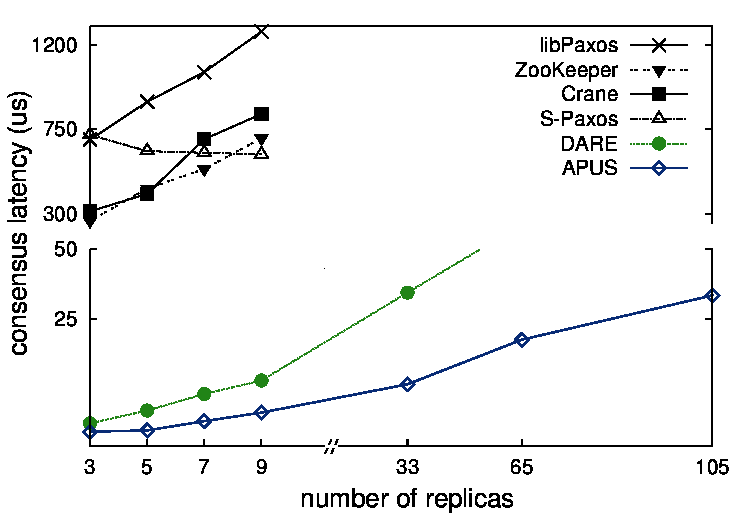
\includegraphics[width=0.25\textheight]{figures/traditional_paxos_latency.ps}
%         \vspace{-.2in}
%         \caption{Consensus latency of six \paxos protocols. \falcon is fastest 
% and scales the best.}
%         \label{fig:scalability}
% \end{figure}


% When changing the replica group size 
% from 3 to 105 (a 35x increase), \falcon's consensus latency increases merely 
% from \xxxlatencythree \us to \xxxlatencyonezerofive \us (a \xxxscalability, 
% sub-linear increase).
% Crane. Falcon. Say Crane is first version. Falcon 
% totally subsumes Crane. Falcon also has initial results.



\para{Future work.} We will further improve the practicality of \kakute in two 
dimensions. First, we will extensively evaluate its performance on broad 
big-data programs. Second, we will leverage it to improve existing security 
techniques, including anonymization techniques and diff privacy (Objective 2). 

\vspace{-.15in}\subsection{Objective 2: 
fine-grained diff privacy}\label{sec:obj2}\vspace{-.075in}

We are proposing
to combine IFT and differential privacy. With IFT, security levels are 
propagating
throughout computation, while differential privacy is for preventing individual 
information leakage.
In this model, different records and fields can have various security levels,
therefore, a general and fine-grained differential private framework can be 
achieved.
Programmer does not need to modify their analysis programs and tradeoff between
usability and security can be achieved with different users.

It needs to determine the relation of the privacy budget and the security
level.
In a simplest model, there are 5 security levels: insensitive, dp-1,
dp-2, dp-3, non-released. Insensitive record can be release directly,
while non-released can not be used in
any computation to the final result. dp-1 to dp-3 varies in terms of their
privacy budgets for differential privacy.
We may also consider the $(\delta, \varepsilon)$-differential privacy model.

% \subsection{Security level and accuracy, and usability analysis}
% 
% \subsection{Range Estimation}
To estimate the range of a output, so that the laps noise distribution
can be determine by running the same, differentially private percentile 
estimation algorithm on the inputs to compute the 25-th and the 75-th 
percentile privately (a.k.a, lower and upper quartiles) for the inputs.

% \subsection{Noise Aggregation}
We extend the differential privacy model developed in previous
work~\cite{differentialdp:stoc11}. We introduce two noise aggregation model
that make use the fact that different record may have
different security level (protection level).

% \subsubsection{Naive Aggregation Model}
A simplest model is to use the $\varepsilon$ inferred by the highest security
level, then add noise to the output directly.
Add noise to the output with $f(x) + Lap(\dfrac{max - min}{\varepsilon_{max}})$.
This simple model may generate two much noise to the final result, which
make the result unusable. The complete algorithm is showed in 
Algorithm~\ref{algo:naive}.

\begin{algorithm}[t]
\SetAlgoLined
\KwIn{Dataset T, dataset size N, privacy budget $\varepsilon_k$ for security 
level k,
  output range (min, max)}
  n = 4

 \For{$i\leftarrow 1$ \KwTo $n$}{
    $O_i$ $\leftarrow$ $f(T_i)$\;
    if $O_i$ > max, $O_i$ $\leftarrow$ max
    if $O_i$ < max, $O_i$ $\leftarrow$ min
 }
 \For{dimension $j$ of the output $O$}{
    k $\leftarrow$ $max(getLevel(O_{j}))$\;
    $O_j$ $\leftarrow$ $\dfrac{1}{n}\sum\limits_{i=1}^n O_{ij} + Lap(\dfrac{max 
- min}{\varepsilon_{k}})$
  }
  \KwOut{$O$}
 \caption{Naive Aggregation Model}
 \label{algo:naive}
\end{algorithm}

% \subsubsection{Combined Aggregation Model}
In this model, data is partitioned into multiple parts (size of each part is 
$m$). Each partition may consists
different level. The noise aggregator adds noise to final result of each 
partition
according to the security level of each partition.

Formally, data is partitioned into multiple parts denoted as $p_1$, $p_2$, ..., 
$p_n$.
The security level and its corresponding $\varepsilon$ are $\varepsilon_1$,
$\varepsilon_2$, ..., $\varepsilon_n$. Therefore, the final aggregated result
is

\begin{align}
\dfrac{\sum\limits_{i=1}^n f(x_i) + Lap(\dfrac{max_i - 
min_i}{\varepsilon_i})}{n}
\end{align}

The complete algorithm is showed in Algorithm~\ref{algo:combined}.

\begin{algorithm}[t]
\SetAlgoLined
\KwIn{Dataset T, dataset size N, privacy budget $\varepsilon_k$ for security 
level k,
  output range (min, max)}
  n = 4

 \For{$i\leftarrow 1$ \KwTo $n$}{
    $O_i$ $\leftarrow$ $f(T_i)$\;
    if $O_i$ > max, $O_i$ $\leftarrow$ max
    if $O_i$ < max, $O_i$ $\leftarrow$ min
    \For{dimension $j$ of the output $O$}{
       k $\leftarrow$ $max(getLevel(O_{ij}))$\;
       $O_{ij}$ $\leftarrow$ $O_{ij} + Lap(\dfrac{max - min}{\varepsilon_{k}})$
     }
 }
 \lForEach{partition $i$ of the output $O$}{$O_j$ $\leftarrow$ $ 
\dfrac{1}{n}\sum\limits_{i=1}^n O_{ij}$}
  \KwOut{$O$}
 \caption{Combined Aggregation Model}
 \label{algo:combined}
\end{algorithm}

The error of the final result incurs in this aggregator comes from two parts:
the Laps noise error and the partition error. It is crucial to reduce the final
error incurs by this aggregator while keeping the differential security 
guarantee.
The error of this model (when the eps is the same) is

\begin{align}
|\dfrac{1}{n}\sum\limits_{i=1}^n f(T_i) - f(T)| + 
\dfrac{1}{n}\sqrt{2}\bigtriangleup{f}\sum\limits_{i=1}^n\dfrac{1}{\varepsilon_i}
\end{align}, and it should be minimized.
% TODO: do this model

As final result of each partition may consist
different security levels, the final noise can be less than previous method.

If we can get the statistic of security levels, we can estimate the block
size in a better way. In specific, suppose there are k security levels and
$M_k$ means that $M_k$ partitions has a maximum security level as k. The the
above equation can be rewritten as
\begin{align}
  |\dfrac{1}{n}\sum\limits_{i=1}^n f(T_i) - f(T)| +  
\dfrac{1}{n}\sqrt{2}\bigtriangleup{f}\sum\limits_{i=1}^k\dfrac{1}{\varepsilon_i} 
* M_i
\end{align}
$M_k$ can be calculated according to the total partition number $n$ and
the number of block that has security level as $k$ (denoted as $p_k$), then
we can further formulate it as:

% directly save the odp file to eps, level 2.
% \vspace{.1in}
% \begin{figure}[!htb]
% %     \centering
%     \begin{minipage}{.48\textwidth}
%         \vspace{-.3in}
%         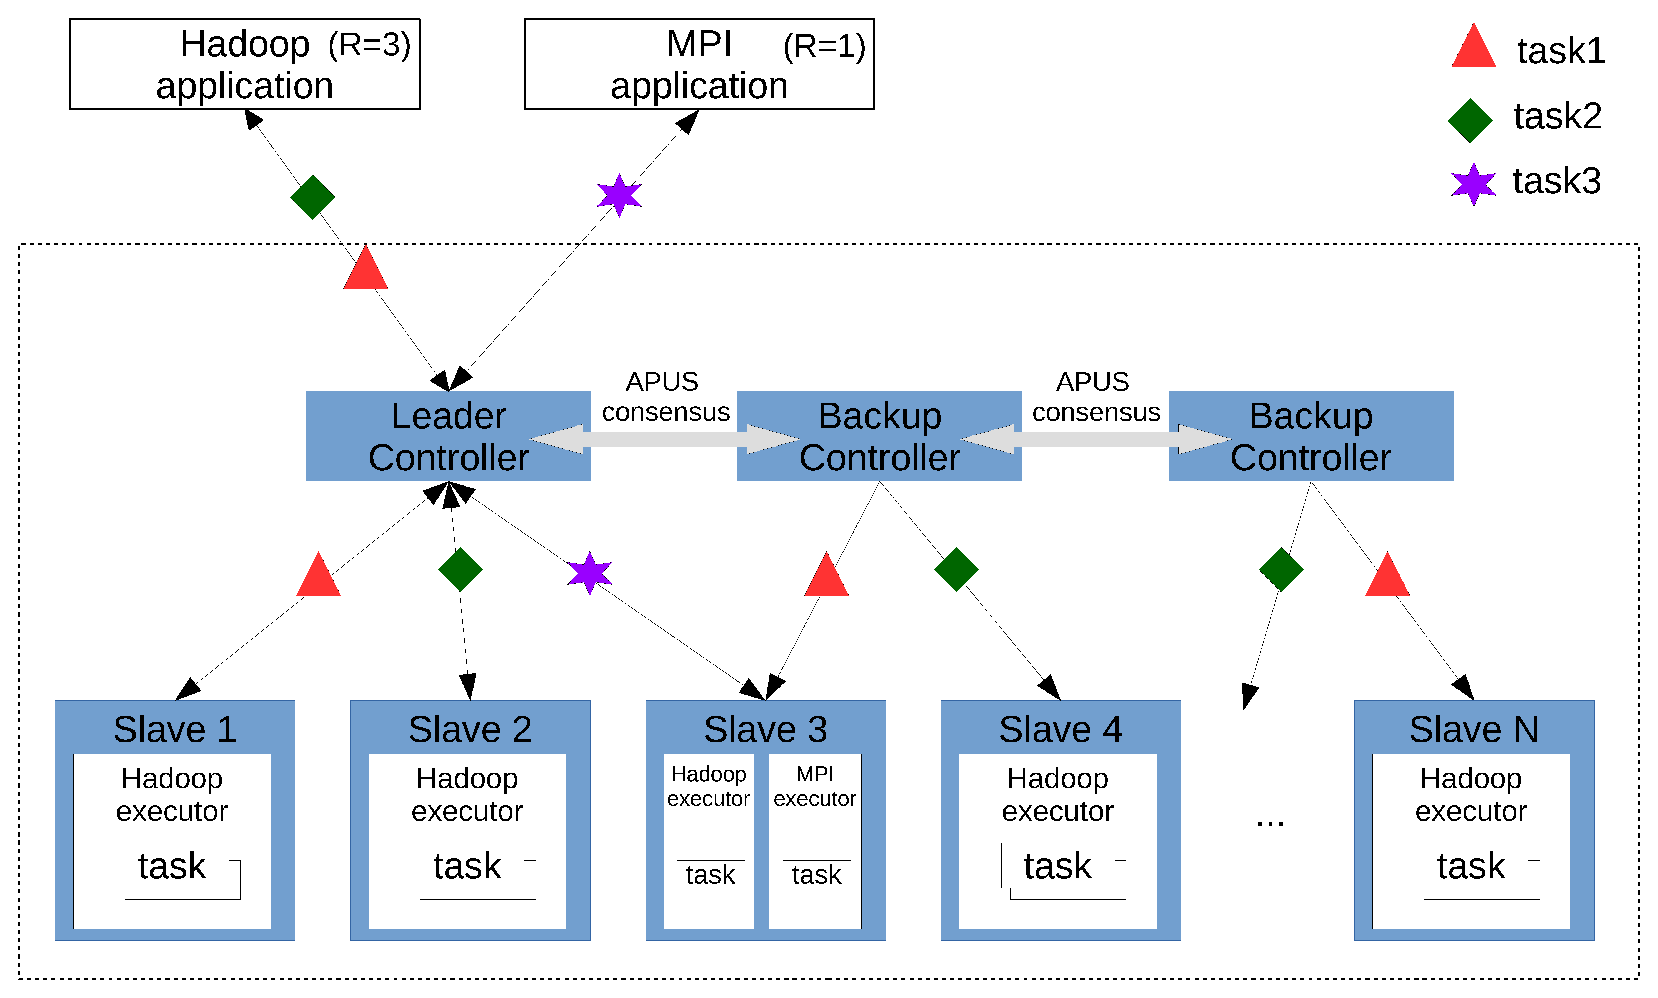
\includegraphics[width=0.34\textheight]{figures/scheduler_arch.eps}
%          \vspace{-.4in}
%         \caption{\tripod scheduler architecture. It replicates all 
% Hadoop~\cite{hadoop} tasks (\vv{R=3}) for fault-tolerance and runs all 
% MPI~\cite{mpi} tasks as is (\vv{R=1}).}
%         \label{fig:scheduler-arch}
%     \end{minipage}
%     \hspace{0.16in}
%     \begin{minipage}{0.48\textwidth}
%         \vspace{-.3in}
%         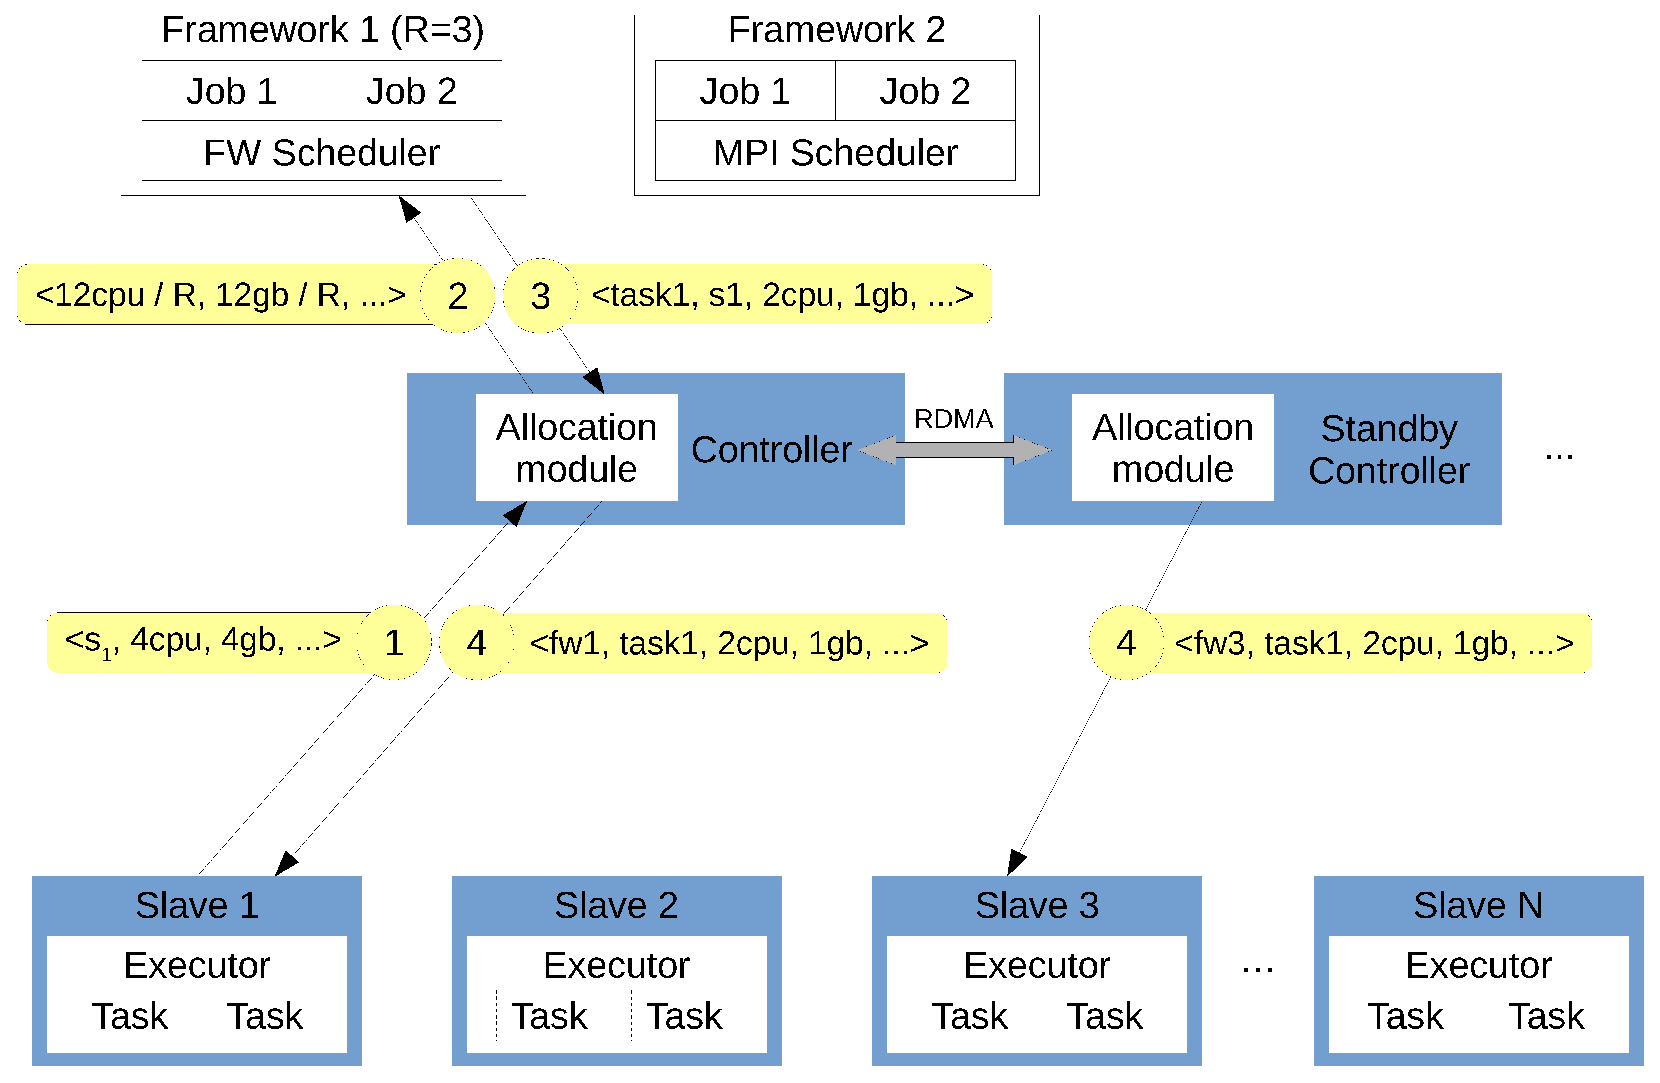
\includegraphics[width=0.34\textheight]{figures/scheduler_flow.eps}
%         \vspace{-.4in}
%         \caption{The replication-aware resource allocation scheme with four 
% steps (\textbf{S1}$\sim$\textbf{S4}).}
%         \label{fig:scheduler-workflow}
%     \end{minipage}
% \end{figure}



\vspace{-.15in}\subsection{Objective 3: building a 
secure just-in-time compiler}\label{sec:obj3}\vspace{-.075in}


In the project, we plan to tackle the problem above. We are proposing to
run unmodified Java program in enclaves to protect computation in public
clouds or untrusted servers. We will design a Just-In-Time compiler for JVM
and run secured functions in enclaves.\\
\textbf{Thread Model} We evaluate the program setup in public clouds.
In a public cloud, only data provider, and a portion of code
in the analytic platform
that is running in the enclaved are trusted. In specific, the JIT compiler and
the secure functions should be trusted.
All other components, including operating system,
hypervisor are trusted. Figure~\ref{fig:threat_public} shows the model (TODO).
\begin{figure}[!h]
  \center
  \footnotesize
  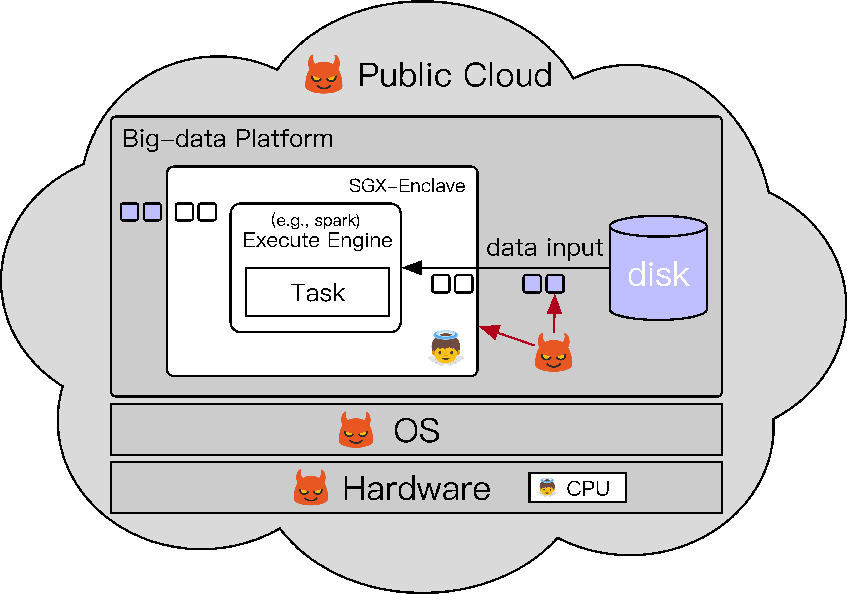
\includegraphics[width=0.5\textwidth]{figures/threat_public.ps}
  \caption{\footnotesize{Threat model in public cloud. All grey boxes are not 
trusted and red lines
  represent potential leakages or attacks. Data is encrypted outside enclave and 
is in blue.}}
  \label{fig:threat_public}
\end{figure}

Figure \ref{arch} shows the architecture
of the system. Programmers annotate some functions as secure, so code of the 
functions
and data processed by these functions should be kept as secrets.
The annotated secure functions are compiled and executed inside
enclaves so that data and code will not be leaked.
The Java byte-codes of these function are compiled to native enclave
codes, and are executed inside enclaves upon function calls.

\begin{figure}[tbh]
  \center
  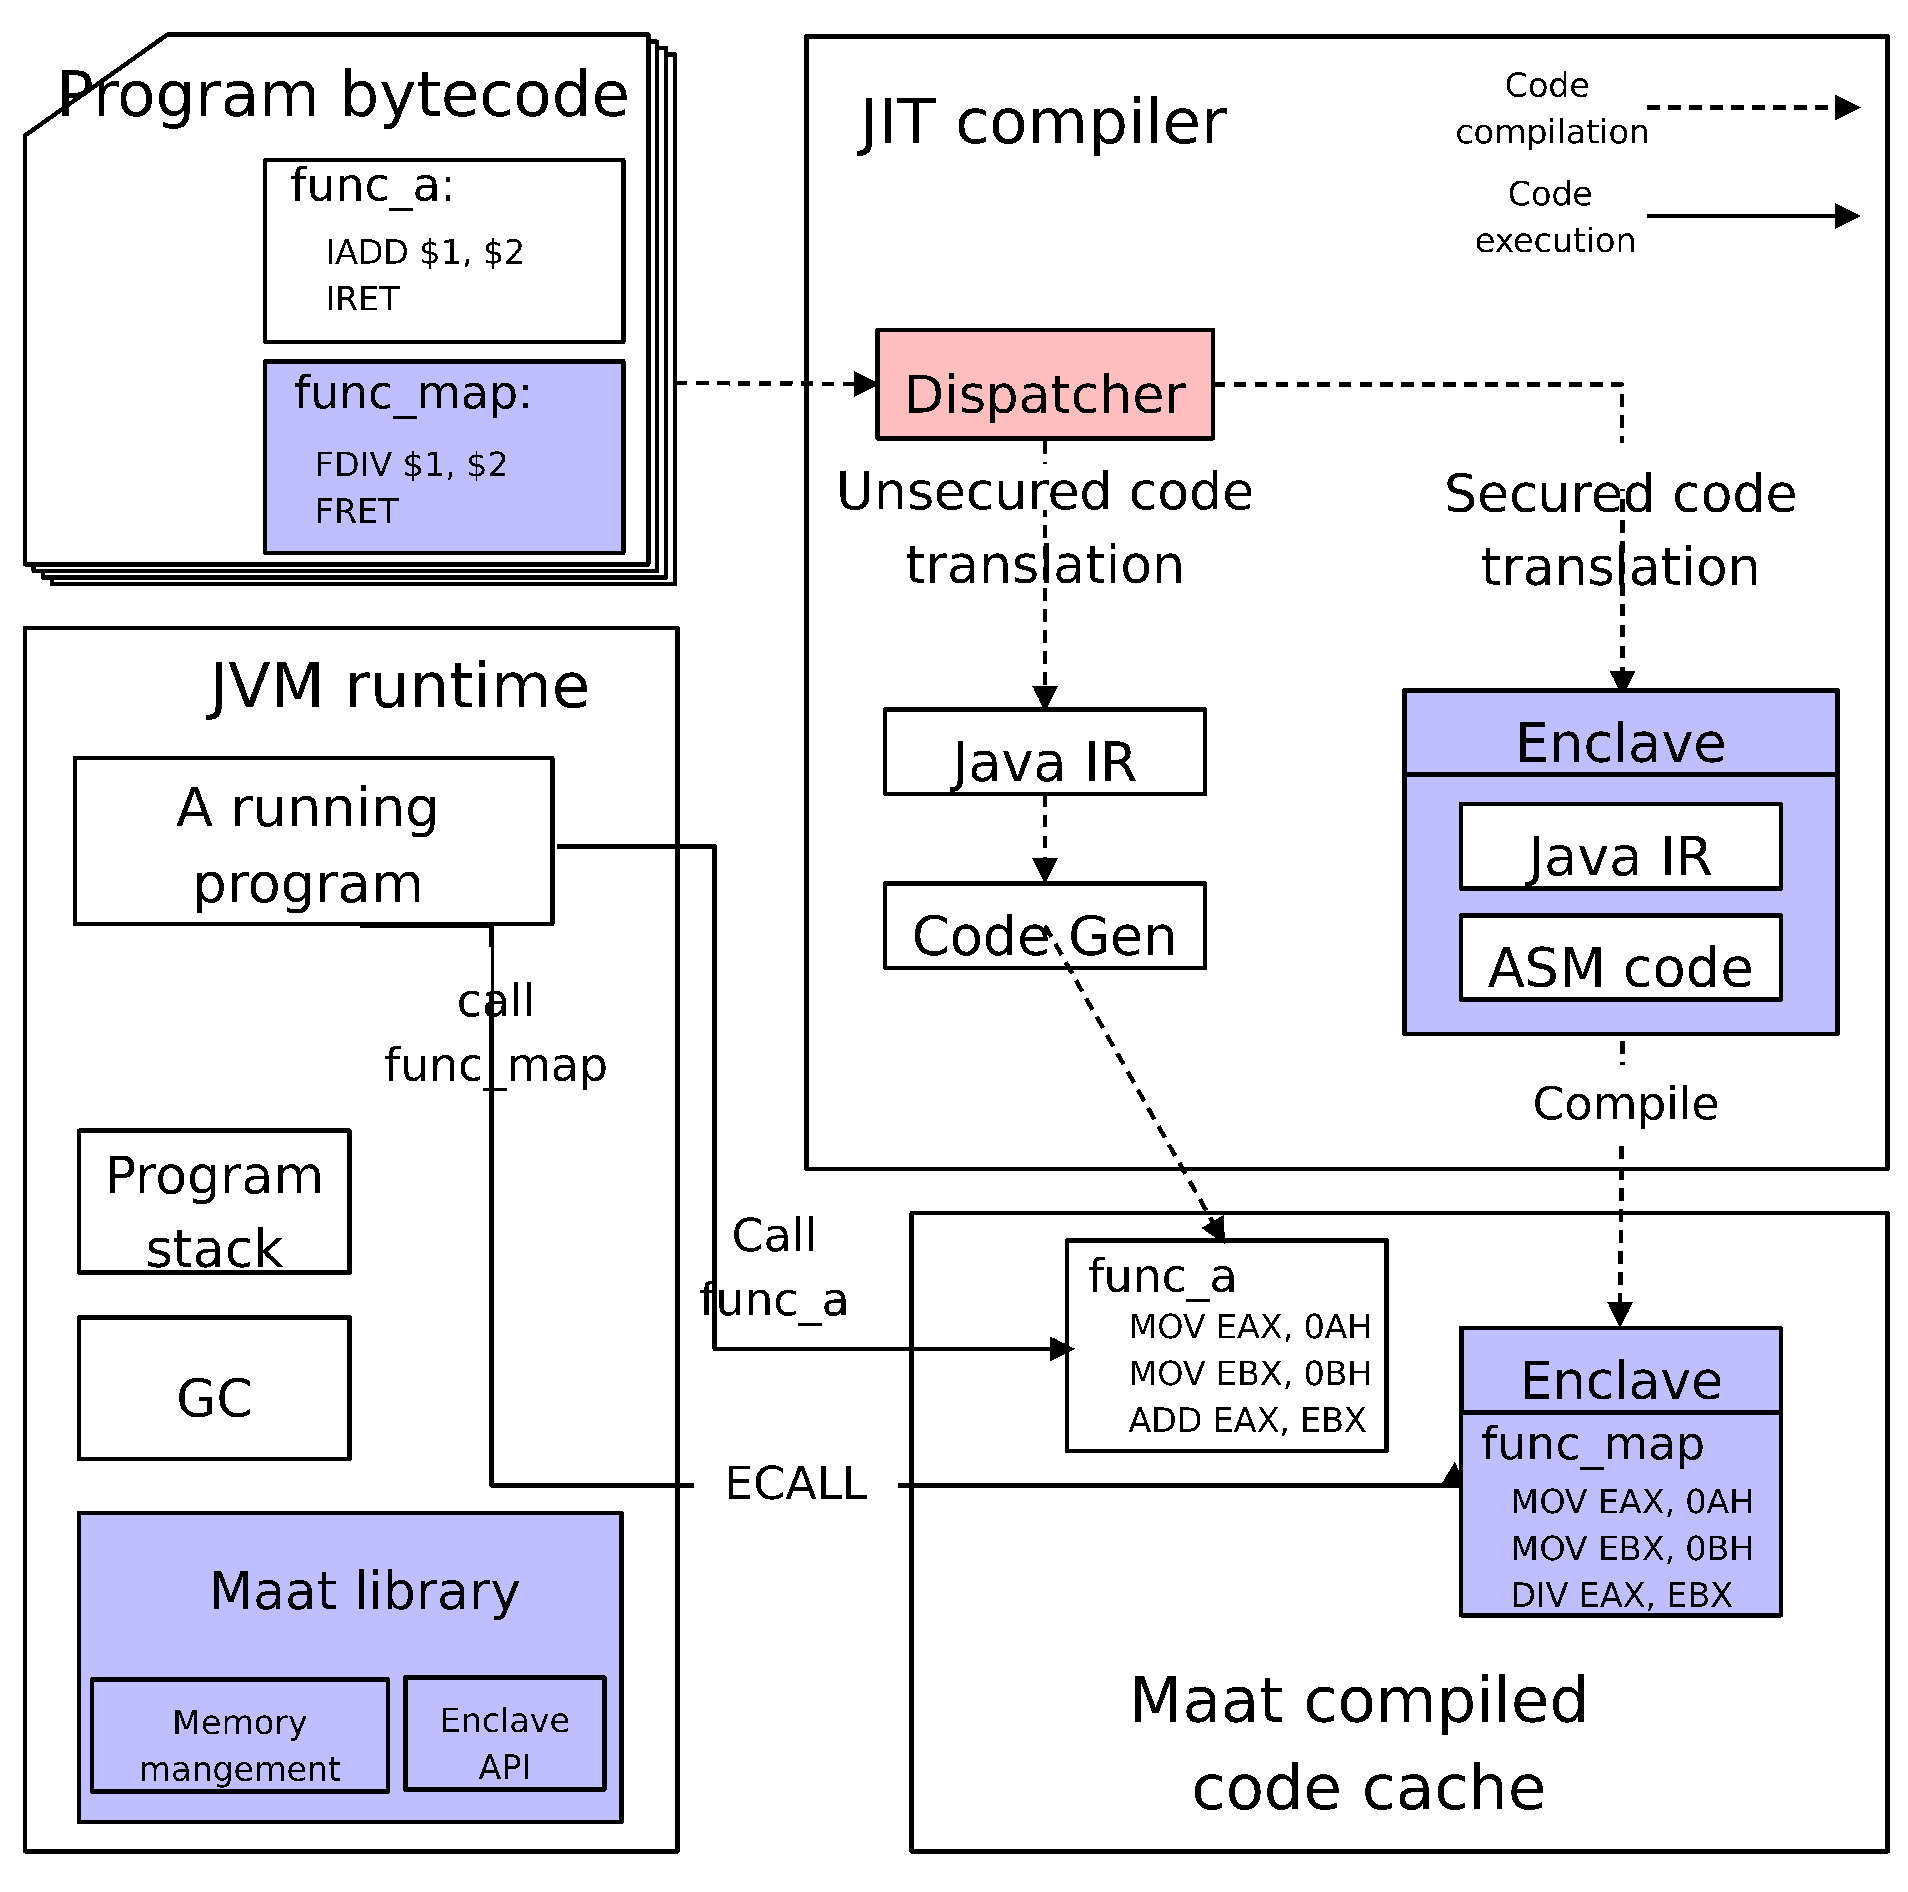
\includegraphics[width=0.75\textwidth]{figures/jit_arch.ps}
  \caption{Architecture of Running Java with SGX. Some of the functions are
  annotated as secured function and they are compiled by a JIT in a enclave.
  The compiler compiles the functions into enclave code, so that the program 
will
  call into a enclave when calling into this function.}
  \label{arch}
\end{figure}

There are two challenges that we need to address in our design:
running unmodified Java programs with minimum TCB and
reducing excessive enclave transitions.

% \subsubsection{Running Unmodified Java Programs with Minimum TCB}
A straightforward approach to run unmodified Java programs in enclaves for
code and data protections is to run the whole JVM in enclaves.
However, as argued in a previous work~\cite{securekeeper},
it will blow up the TCB and cause a high overhead by running the whole JVM in 
enclaves.

% TCB
SGX is for protecting data and code running in enclaves, but code inside 
enclaves
also have accesses to the regular memory region. Therefore, code in the enclaves
can write sensitive data to unprotected memory regions when the code is 
compromised.
The OpenJDK implementation of JVM contains up to millions lines of code, which
is unpractical for formal verifications as it is time-consuming with
current verification methods (\chref{sec:others-work}).

% Memory size
Intel SGX contains a protected memory region call Enclave Page Cache (EPC), and 
evictions
from this cache cause expensive encryption costs.
Although next generation of SGX~\cite{intel-sgx2} may support a larger EPC,
current generation of SGX only has an EPC up to 128MB. In practice, only around
90 MB can be allocated. Therefore, running programs with large memory 
consumption
will cause much higher overhead. A recent work~\cite{opaque:nsdi17} shows that
running program below this limit incur an only 7.46\% overhead, while slightly
exceeding this limit causes 50\% to 60\% overhead.
Therefore, we have to reduce the TCB size for running unmodified Java programs
in enclaves.

To reduce TCB size, we propose to run only some programmer-annotated functions
in enclave. To this end, we propose a split execution framework.
Only the Intermediate Representation (IR)
and Code Generation model are trusted in the system. There will be two instances
of compilers for compiling Java bytecode, one for secure code compilations and 
one
for untrusted code compilations. Therefore, the TCB is greatly reduced, as we
do not need to trust the JVM runtime (\eg{} Garbage Collection). Also, as only
some functions should be executed securely, the split execution framework
should not cause high performance overhead.

When calling into and out of a function in enclaves, an ECALL and OCALL
will be invoked in the CPU. In specific, the CPU is trapped into a new mode 
(except from
the User and Privileged mode), and the current frame is encrypted and saved.
A recent work~\cite{sgxkernel:cf17} shows that enclave transitions are 60X 
slower
than system calls and several hundreds times slower than user function calls.
Moreover, encryption and decryption are required for secure function calls,
which makes enclave transitions even more time-consuming.
Our evaluation on a recent privacy-preserving data analytic 
system~\cite{opaque:nsdi17} shows that
it incurs 3.4k transitions for processing 10k data (for two operations select 
and groupBy).
In fact, these processing functions can be pipelined and processed in a single
enclave function. Our project takes reducing transitions as one of our targets.
% Therefore, system with frequent enclave transitions would have high

We introduce two techniques, Cost-based Compilation and Asynchronous
Enclave Call, to tackle this challenge.
Cost-based Compilation can make use of the JVM hotspot features, and analyse
the hotspot enclave functions. It builds a tree of callers and callee of 
functions,
and combines two enclaves if the marginal benefit of combining them is larger 
than
the transition cost. Initially, only function b and d
are running in enclaves, but the compiler finds out that cost of running c in an 
enclave is less than the transition cost (assume it to be 2), then the whole 
function a will be compile as an enclave. In another case where running 
function c takes a high cost, combinations of enclaves will not happen.
Therefore, transition of enclaves can be reduced. This technique can be applied
online or offline. In a offline version, it sample the program and finish the
optimisation offline.
% % Figure~\ref{on-time} shows the example. 

Asynchronous Enclave Call convert the synchronous enclave calls to asynchronous
enclave calls. In specific, when a secure function is called,
the function call and its parameters are put into a QUEUE which will be fetch by
the enclave can be executed. After finishing execution, the result will be 
stored
in QUEUE\_R and the current execution will resume and continue. 
This technique makes use of the multi-core
hardware architecture and enclaves and the main program are running in separate
threads.
% Figure~\ref{asynccall} shows the idea of this technique. 

These two technique can be applied simultaneously, the compiler can run the
sample and optimisation offline. After that, the compiler run a enclave and the 
program
in separate threads to avoid transition of enclaves.

% \para{Oblivious Execution}. Our current design does not consider data leakage 
% through access pattern, but
% recent work~\cite{access:pattern:ccs15, access:pattern:ndss12} has showed
% that access pattern can leak a significant amount of
% sensitive information. Intel SGX does not provide protection for access pattern,
% and attackers can get the code paths
% or data access patterns inside the enclave by side channel
% attacks~\cite{sgx-explain}.
% 
% Oblivious Ram~\cite{oram:jacm96, hashoram:soda12,oram:soda12, pathoram:ccs13, 
% circuit:oram:ccs15}
% is proposed to prevent access pattern leakage, but they need to modify the
% original program. ObliVM~\cite{oblivm:sp15} is a programming framework for 
% writing
% programs with oblivious
% executions, and it provides a convenient programming language for writing 
% programs.
% Oblivious Data Structure~\cite{obli:data:ccs14, obli:data:asiacrypt14} provides
% efficient oblivious implementation of data structure such as queue, and so on,
% which is useful for writing oblivious programs. A previous 
% work~\cite{autooram:sp14} automatically
% translate a program to a oblivious implementation.
% 
% To support oblivious execution for Java programs, we can further
% extend the secure compiler for compiling a Java program to a oblivious native
% code, including replacing the branch, loop operations to oblivious operators
% and making use of the oblivious data structure abstraction.
% % It can compile the a program% to a sequence of circuits.
% Therefore, this secure abstraction will be a strong abstraction for
% secure computations.
% 
% \para{Support System Calls in Enclaves}. Our current design focus on supporting 
% secure data analytic programming, so
% it does not provide support for system calls. We aim to support system
% calls in the future.
% 
% We plan to adopt a combination of emulation and delegation design of system call
% handling like a
% previous work~\cite{sgxkernel:cf17,graphene:atc17}. Emulation of system calls
% reduce cost of enclave transition, while delegation can reduce TCB size. We will
% adopt emulations for simple but usually used system calls. We believe this
% hybrid design can accomplish a fast but secure system handling in Java.

\vspace{-.15in}\subsection{Research timeline} 
\label{sec:timeline}\vspace{-.075in}

This project will require two PhD students S1 and S2 to work for 
three years. In the first year, S1 will design and fully implement the \kakute 
system (part of \textbf{Objective~1}), and S2 will evaluate its performance 
and robustness on various real-world big-data queries (part of 
\textbf{Objective~1}). In the second year, S1 will 
use \kakute to fully develop the proposed fine-grained privacy model (part of 
\textbf{Objective~2}), and S2 will implement the two algorithms proposed for 
this model (part of \textbf{Objective~2}). In the third year, S1 will build the 
secure big-data compiler \textbf{Objective 3} and S2 will evaluate this 
compiler on diverse real-world big-data queries.
% Both students will 
% involve theoretical methods, implement real software systems, and 
% perform real-world study.
% The PI will supervise the students by providing 
% advice concerning both theoretical and systems implementation levels.


